
\subsection{BLEビーコンのアプリケーション化とBLEビーコンを併用したシステム}

BLEビーコンの導入は容易だが,可用性,ユーザの利便性に問題がある.
BLEビーコンの電池がなくなると,ビーコンの動作が停止する.在室情報を継続的に記録するには,ビーコンは常に動作する必要がある.
そのためビーコンの電池切れになった際はユーザに電池交換するように促しを行っていた.
しかし,電池交換がされない状況が存在した.
なぜならBLEビーコンの電池切れを気づくのが困難だからである.
BLEビーコンの電池残量の把握は専用のアプリケーションによる接続が必要であるため,事前にユーザが電池切れを防ぐことは難しい. (説明が必要かも)
またBLEビーコンの電池切れに気づいたとしても,電池交換はユーザに委ねられている.
この電池交換は少し手間がかかる.
そのため電池交換をされずに電池切れを起こしたままのビーコンが放置される状況が存在した.

そこで可用性向上,ユーザの利便性向上のために,BLEビーコンのアプリケーション化をした.
(ここに説明を書いて欲しい どういう風にアプリケーション化したか,kotlinとかペリフェラルとかその辺の説明  亀田)

アプリケーション化に伴い可用性はハードウェア面,ソフトウェア面から改善がされた.
ハードウェアとして動作するスマートフォンはユーザが高頻度で状態を確認するため,バッテリー切れなど状況の判別が容易である.
また,スマートフォン自体の可用性を維持するために対策を講じるユーザが多く,ビーコンと比較してハードウェアとして可用性が維持されやすい.
ソフトウェア面では,図2に示す通りスマートフォンの通知領域に動作状況を可視化する.
通知領域への表示はビーコンとしての動作と連携しており,アプリケーションの動作中は永続的に表示される.
よってアプリケーションが停止した場合もユーザによる判別が容易であるため,アプリケーション再起動によって可用性が維持されやすい.

\begin{figure}[tbh]
  \centering
  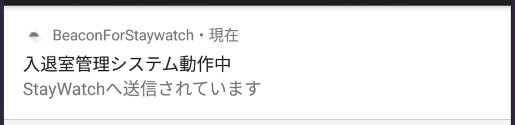
\includegraphics[width=8cm]{image/notify.jpg}
  \caption{通知領域による可視化}
  \label{multipleBPM}
\end{figure}

またバックグラウンド動作によってユーザ操作の負担を低減している.
既存のBLEビーコンの利点として正常に動作している限り,ユーザの操作が不要である点が挙げられる.
アプリケーション化に伴い,ユーザの操作が必要になったがそれを最小限に抑えるため,バックグラウンド動作による負担低減を行った.
ユーザの必要な操作は初回のみ必要なログイン処理とビーコン動作の切り替え処理のみである.

またこのスマートフォンアプリケーションとBLEビーコンをハイブリット化して利用することで色んな属性のユーザが継続的に利用できる.
普段から継続的に使ってる滞在ウォッチユーザにとっては,BLEビーコンは上で述べたように電池交換の手間がある.
スマートフォンアプリケーションはそのようなユーザにとっては,電池交換の手間がないため有用である.
しかしスマートフォンアプリケーションはアプリのインストールに抵抗があるユーザやインストールができないユーザも想定される.
例としてはスマートフォンを持っていないユーザ,アプリの使用に伴うバッテリーの消費気が気になるユーザなどが上げられる.
これらの問題はBLEビーコンとスマートフォンアプリケーションをハイブリット化することで解決できる.
スマートフォンアプリケーションをBLEビーコンのUUIDと同じにしてどちらでも同じユーザの在室情報を記録している.
この方法はスマートフォンのアプリかBLEビーコンのどちらかを持っていればよいため継続的にデータを記録する観点から見ても有用である.














